\chapter{相关工作综述}
电子表格的相关工作主要集中在两个研究领域,信息系统和计算机科学领域。
在本章中,我们从计算机科学领域(主要是软件工程)的视角出发,对电子表格的质量保障技术进行分类讨论。
根据它们的设计目的,我们把各种电子表格的质量保障技术分成两类:
\begin{itemize}
    \item \textit{避免错误}的技术帮助终端用户从开发的起始阶段就能创建出不含错误的电子表格,对应本章第一节讨论的相关工作;
    \item \textit{发现和修复错误}的技术帮助终端用户检测电子表格中蕴含的错误并理解错误发生的原因,进而修复这些的错误。
    这类技术通常在电子表格已经开发、编辑完成之后使用,对应本章第二节和第三节讨论的相关工作。
\end{itemize}

接下来,我们将相关工作分成三个小节来讨论,即模型驱动的电子表格开发技术、电子表格的缺陷定位、检测和修复技术、以及电子表格的辅助支撑技术。


\section{模型驱动的电子表格开发技术}
基于模型驱动的方法并不是设计用来帮助终端用户发现潜在的错误,而是把提升电子表格的质量、结构的清晰度和防止错误注入放在首位。
类似于一般软件工程领域的模型驱动方法,这类技术的核心想法是在电子表格的开发过程中引入额外的抽象层。
这个额外的抽象层引入了更多抽象概念,在开发者的内在意图和电子表格的真实实现中间充当了沟通的桥梁。
在商业化的电子表格系统中日益扩大的这层语义鸿沟\cite{luckey2012systematic}得到了有效缓解。

这类抽象的电子表格模型通常出现在开发过程的两个阶段:
\begin{itemize}
    \item 它们被用作“代码生成器”的形式化描述。在这个场景下,电子表格的一部分从模型中自动生成,因此减少了纯人工操作产生错误的风险;
    \item 它们也被用于从已有的电子表格中恢复出内在蕴含的概念结构,帮助终端用户理解当前电子表格的计算模型,进而减少后续可能产生的误解。
\end{itemize}

\subsection{电子表格的面向对象模型}
Isakowitz 等人\cite{isakowitz1995toward}是最早提出从建模角度来处理电子表格程序。
他们的核心假设是电子表格程序可以看做物理和逻辑的两个部分,物理部分就是单元格的公式和数值,逻辑部分就是描述电子表格功能的一系列函数关系。
而逻辑这部分可以从给定的电子表格中自动提取出来,并用领域特定语言(Domain-specific Language,DSL)表达出来。
该系统也能够从这样的逻辑规约中合成电子表格。

Paine 等人\cite{ireson1997model,paine2008ensuring}也提出了类似的针对电子表格程序的面向对象概念。
在他们的 Model Master 方法中,电子表格以声明式的方式表达为文本程序。
这些程序通过编译器处理,随即从规约中生成电子表格。
电子表格的逻辑以类的形式表达,其中包括属性和计算逻辑。
该建模语言中也提供许多特征(如类继承,多维数组扩展)来支持表格化的计算。
我们也可以逆向使用该方法,从给定的电子表格中提取出对应的逻辑模型,进而用于发现电子表格中的特定计算结构\cite{paine2008spreadsheet}。

Paine 等人\cite{paine2005bringing,paine2008rapid}后续提出了另一种声明式建模语言。
他们开发的 Excelsior 是一个电子表格开发系统,构建在 Prolog 上的编程语言,同时针对 Excel 设计了模块化和可重用的规约表达方式。

\begin{figure}[tp]    
    \centering
    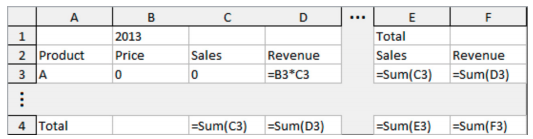
\includegraphics[width=1\textwidth]{figure/template.png}
    \caption{电子表格模板示例}
    \label{figure-template}
\end{figure}
\subsection{电子表格的可视化模板}
Erwig 等人\cite{erwig2004gencel,erwig2005automatic,abraham2005goal}提出基于表格模板的可视化方法来刻画电子表格底层模型的特定方面。
在他们的 Gencel 方法中,一个“表格模板”被用来特指电子表格中重复的区域。
图\ref{figure-template}展示了一个可视化模板的例子。
模板的设计和修改过程类似于 MS Excel 软件的可视化操作方式。
在图\ref{figure-template}中,$B$、$C$和$D$列下面的内容被标记为可重复的。
这类可重复的区域用所在列上和所在行上的两个省略号"..."和两条分隔带来表达。

类似于 Paine 等人的工作,电子表格也可以从模型中自动生成。
另外,基于模板的方法也支持逆向工程,Abraham 等人\cite{abraham2006inferring}提出使用一些启发式方法能够从给定的电子表格中自动提取出存在的模板。

后来,Engels 等人\cite{engels2005classsheets,cunha2010automatically}结合基于模板的方法和面向对象的概念模型提出了 ClassSheet 的概念,
突破了基于模板方法只能刻画电子表格的“词法特征”的局限性,使用 ClassSheet 概念能够更完整地刻画整个表格的“语义特征”。
许多基于 ClassSheet 概念的改进方法被陆续提出\cite{luckey2012systematic,cunha2011type,cunha2011embedding,cunha2012bidirectional}。
比如 Luckey 等人\cite{luckey2012systematic}处理了模型演化和如何使得这类更新能够自动转换到已经生成的电子表格中的问题,以便更好地支撑电子表格完整的开发过程。

Hermans等人\cite{hermans2010automatically}提出了另一个不同的可视化方法来重构底层面向对象模型。
该方法基于人工设计的经典模式库,通过二维解析和模式匹配算法来尝试定位电子表格中的各类构建模式。
最终的构建模式被转换成 UML 类图,可用于更好地理解和提升当前的电子表格质量。

\subsection{电子表格的关系型模型}
电子表格的主要原则之一:数据以表格的形式组织。
一个直接的获得表格的结构模型的方法是借鉴关系型数据库的设计原理和实践方法。
以构建高质量和零错误的表格为目的,Cunha 等人\cite{cunha2009spreadsheets}提出了从电子表格中提取关系型数据库范式的方法。
该方法的主要优点是能够获得更加模块化、没有数据冗余、并预防错误的数据输入的电子表格模型\cite{cunha2009discovery,cunha2012relational}。


\section{电子表格的缺陷分析技术}
电子表格的编程范式使得终端用户容易犯错。
随着电子表格包含的数据量越来越大,依赖终端用户人工检查每个公式的计算结果是否符合预期,效率低下。
相应地,针对电子表格的自动化错误/缺陷定位、检测和修复工作得到了研究者们的广泛关注。
这些方法也可以基于是否需要人工辅助分成两类,人工辅助具体包括用户给定测试输入、按要求提供额外的标注信息等。

\subsection{缺陷定位}
早期的电子表格错误定位工作\cite{reichwein1999slicing,ruthruff2005interactive},使用计算轨迹的候选者排序策略来寻找有缺陷的单元格,类似于传统程序分析中的基于频谱的错误定位方法。
他们首先提出将程序切片的概念应用到电子表格中,以消除不可能的错误候选者。
该类技术使用用户给定的辅助信息关于正确和不正确的单元格值,并把对一个错误的单元格值有贡献的单元格标记为可能错误的。
一个单元格的公式如果对更多的已经标记为错误的值有贡献,那么很可能就是错误的。
相反,对更多正确的单元格值有贡献,那么很可能就是正确的。
如果一个单元格对错误的单元格值有贡献,但是它本身只由正确的单元格值计算而来,那么它的错误可能性就会减小。
该类方法,就是依据这种想法,进行量化排序。
后续,Hofer 等人\cite{hofer2013empirical}使用更加形式化的方法,以相似性系数来计算电子表格单元格的错误可能性。

另一条错误定位的思路是把电子表格转换成基于约束的形式,使得关于异常值的原因定位的复杂推导变得可能。
Jannach 等人\cite{jannach2010toward}提出将电子表格错误定位问题转换成约束可满足性问题(CSP)\cite{tsang2014foundations}。
基于用户给出的测试用例和关于某些单元格的异常值信息,该方法使用基于模型诊断的原则来判定哪些单元格原则上可能是异常计算结果的真正原因。
后来,Jannach 等人\cite{jannach2016model}又提出了新的算法改进策略,帮助提升原方法的可扩展性。

类似的方法也得到了 Abreu 等人\cite{abreu2012constraint,abreu2012debugging}的采用。
Abreu 的方法尽管整体上与 Jannach 等人的方法相似,但技术实现上有差异。
他们没有使用 Hitting-Set 算法\cite{reiter1987theory},而是把单个公式的正确性的推导直接编码成约束表达。
因此他们利用了额外的布尔变量来代表每个公式的正确性。
另外他们的方法可以同时运用于多组测试用例的并发执行。

Hofer 等人\cite{hofer2013empirical}提出把一个轻量级的基于模型的调试技术,结合到他们的基于频谱的错误定位方法中。
他们建议使用从统计错误定位技术(SFL)得到的系数作为基于模型的调试过程的初始可能性值。

\subsection{缺陷检测}
本世纪的前 10 年主要的缺陷检测相关工作,关注于单位和类型推导的方法\cite{erwig2002adding,burnett2002testing,ahmad2003type,abraham2004header,abraham2006type,abraham2007ucheck,antoniu2004validating,chambers2009automatic,chambers2010reasoning}来检测电子表格错误或缺陷。
这类方法的核心想法是推导出输入单元格的单位信息,进而判断公式中的计算是否符合单位之间的运算法则,类似于普通程序在编译器中进行的静态类型检查。
Erwig等人\cite{erwig2002adding,abraham2004header}最早把这种单位推导系统引入到电子表格的特定错误检测中来。
他们根据表头推导策略和用户标注,推导出所有可能的输入单元格单位信息,进而验证公式的单位运算合法性。

本世纪的 20 年代至今,学界更加关注一类称为电子表格缺陷(Spreadsheet Smell/Defect)的公式错误,该概念派生于软件维护领域的代码潜在错误\cite{fowler1997refactoring},用于特指不良代码设计风格和使用习惯。
这些代码本身未必是错误的,但在未来的软件开发、重构或拓展过程中可能导致错误。
Hermans 等人\cite{hermans2012detecting,hermans2012detecting2,hermans2013data}最早明确地将此类概念发展到电子表格领域中。
通常,电子表格缺陷是通过一些启发式的方法来描述不良设计风格。
Hermans 等人\cite{hermans2012detecting} 提出所谓的“工作表之间的单元格缺陷”。
这类缺陷根据不同工作表之间的依赖关系分析,来识别一些不良使用导致的单元格缺陷。
比如,一个公式引用了很多另一个工作表中的单元格,那么该公式应当被移动到对应工作表中。
公式缺陷最早在\cite{hermans2012detecting2}的工作中得到较为深入的分类和讨论。
后续,Hermans 等人\cite{hermans2013data}提出一个定位电子表格中数据克隆的方法。

窦文生等人\cite{dou2014spreadsheet,dou2017cacheck}提出“单元格阵列”的缺陷检测方法,通过定位同行或同列的具有类似公式语义的连续单元格阵列,进而利用基于组件的程序合成方法在每个单元格阵列中来检测公式异常。
后来,窦文生等人\cite{dou2016detecting}又提出进行跨表格(table)的克隆检测和单元格缺陷检测,通过识别结构同构的表格,进而对相应位置的单元格进行对比,来寻找公式异常。

\begin{figure}[tbp]    
    \centering
    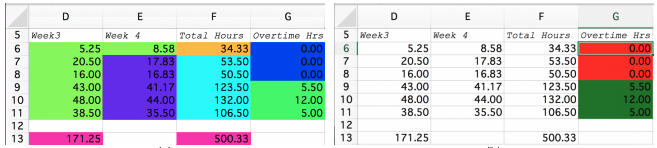
\includegraphics[width=1\textwidth]{figure/figure-excelint.png}
    \caption{ExceLint 工具对公式单元格的划分结果展示}
    \label{figure1}
\end{figure}
考虑到前人工作的召回率偏低问题,Cheung等人\cite{cheung2016custodes}提出基于学习和聚类的技术来对单元格进行分类,尽可能保证每个类中的单元格都含有相似的计算语义,进而在类中检测公式缺陷。
本文即是对 Cheung 等人工作的进一步优化和提升,后面的章节会进一步介绍。
类似地,如图\ref{figure-excelint}所示,ExceLint\cite{Barowy2018excelint}技术通过对公式中蕴含的信息熵分析来给出最合理的电子表格切分方式,最后在每个切分出的单元格矩阵中来进一步检测是否存在公式缺陷。
Melford\cite{singh2017melford}技术通过提取每个单元格附近的其他单元格属性,利用神经网络模型来寻找异常单元格,它的检测范围是\cu \cite{cheung2016custodes}的真子集。

\subsection{缺陷修复}
基于修复的方法不仅向用户指出有潜在问题的公式,也额外给出修复方案,比如应该把错误的公式修改成何种具体的正确公式。
Abraham 等人\cite{abraham2005goal}做出了第一份自动化给出修改建议的工作 GoalDebug(以目标为导向的调试技术)。
该方法中,需要用户为错误的单元格给出预期的结果,通过递归修改单个公式,根据电子表格特定的修改推导规则反向传播到之前的公式中,进而尝试自动给出合适的修改建议。
能够获取预期结果的修改结果再根据启发式方法进行排序。
另一个改进上述提到的 GoalDebug 的方法 \cite{abraham2007goaldebug,abraham2008mutation} 更适合处理多种的电子表格错误类型。
在缺陷检测中提到的工作\ca \cite{dou2014spreadsheet,dou2017cacheck},通过基于组件的程序合成技术\cite{jha2010oracle}也能够为检测到的单元格缺陷提供基础的修复公式建议。


\section{电子表格的辅助支撑技术}
这类辅助支撑技术在电子表格的开发和维护过程中给予用户帮助,包括帮助用户避免发生引用错误、
对电子表格的长期使用提供支撑(监控表格变动的工具、自动化重构的插件等),以及自动帮助用户完成数据提取任务的程序合成工具。

\subsection{演化}
电子表格通常经历各种变化,不巧的是,变化常常会引入错误。
FormulaDataSleuth\cite{bekenn2008reducing}是一个旨在帮助电子表格开发者在表格变动时,立刻检测到这类错误的工具。
一旦开发者已经声明了哪些数据单元格和区域应当被工具监控,系统就会自动监测许多类型的潜在问题。
对于已经定义好的数据区域,工具能够检测出空单元格、或者输入值拥有错误的数据类型、或者超出了预定义的数据范围。
对于被监控的公式单元格,偶然的公式重写以及引用了错误的单元格也会被识别出来。

理解给定的电子表格如何随着时间演化,并观察不同版本之间的差异,对于在不同项目中重用电子表格至关重要。
Chambers 等人\cite{chambers2010sheetdiff}提出了 SheetDiff 算法,能够检测并可视化特定类型的不同版本的电子表格之间的显著差异。
后来,为了克服上述贪心算法 SheetDiff 中存在的问题,Harutyunyan 等人\cite{harutyunyan2012planted}提出一种基于动态规划的算法 RowColAlign,能够更加高效和准确地检测版本差异。
徐良等人\cite{xu2017spreadcluster}利用聚类技术对电子表格整体进行聚类,进而寻找出多个电子表格文件之间的演化关系,并给出了我们在第六章案例研究中使用的测试对象,一个电子表格数据集 VEnron2。

\subsection{重构}
重构被定义为修改程序内部结构,但不修改功能性的过程\cite{o2010spreadsheet}。
除了应用于传统代码,重构在多个方面也有助于电子表格的质量保障。
比如,通过简化公式,使得整体更易理解;通过移除冗余公式,使得维护更加轻松,更少犯错。
电子表格领域的重构通常和行列调整有关,也就是电子表格的设计和布局的转换。
让终端用户人工进行这类转换,常常是耗时且易错的。

Badame等人\cite{badame2012refactoring}根据使用经验提出电子表格中的七种重构策略,并给 MS Excel 软件提供了一个相应的重构插件 RefBook。
该插件自动检测需要重构的单元格位置,并给终端用户提供重构建议。
例如可能提供的重构建议有:将单元格常量化、添加“守护”单元格、以及替换不合理的公式等。

Harris等人\cite{harris2011spreadsheet}提出了一种根据用户给定的样例进行复杂表格转换的方法。
该方法基于一个描述表格转换的领域特定语言 TableProg,以及一个 ProgFromEx 算法。
该算法需要用户提供几组转换示例,描述单元格变化前后的具体字符串。
ProgFromEx 能够自动推导出若干个转换程序,选择其中排序最高的一个,来帮助终端用户完成这样的表格转换过程。
与此类似的相关工作很多,研究者们将程序合成、程序语言领域的理论成果应用到电子表格的实际使用中,如 FlashFill\cite{singh2016transforming}。

\subsection{复用}
通常,复用已有的已经验证过的软件制品能够节约开发时间,避免犯错的风险,提升整体项目的可维护性\cite{ye2005reuse}。
这种复用思路也可以应用于电子表格领域。
独立的电子表格或者其中的部分通常可以在其他项目中重用。
对于公式复用的标准做法是简单的复制粘贴该公式。
然而,改变最初的公式并不会改变它的副本,如果忘记对公式副本进行更新很容易导致错误。

电子表格程序中的复用问题得到了 Djang 等人\cite{djang1998similarity}和 Montigel等人\cite{montigel2002portability}的关注。
Djang 等人\cite{djang1998similarity}沿用了面向对象思想中对继承概念的使用,来实现电子表格中的复用功能。
原则上,它允许用户在单个单元格和更粗粒度的层面上,以多个继承或相互继承的形式,声明电子表格单元格之间的依赖关系。
而 Montigel 等人\cite{montigel2002portability}提出了电子表格语言 Wizcell。
Wizcell 语言通过实现粘贴/复制、拖/拽等功能,使得和复用相关的语义变化更加明显,来缓解复用问题。
%  特别地,提出了四种这类操作的可能输出:
%  要么被复制的公式再被复制一次;
%  要么被复制的公式存在对原公式的引用;
%  要么复制后的单元格中的公式引用了之前原始单元格集合中的某部分单元格;
%  要么其引用随着副本和原来单元格之间的相对距离而对应改变。
Wizcell 语言允许用户声明潜在语义,因此大大降低了由于复用引入错误的可能。


%  \section{电子表格的测试方法}
%  在专业的软件开发流程中,系统测试对于保障软件制品的高质量至关重要。
%  通常这类测试活动既有开发者,也有专门的测试者介入。
%  但因为非专业的电子表格用户通常没有软件工程的思维和实践经验,对应的测试过程通常是不系统且散乱的。

%  考虑到电子表格即时反馈的特质,测试过程通常仅通过输入一组测试用例,然后检查对应的中间单元格和最终的汇总单元格是否产生了预期输出。
%  同时,商业电子表格工具,如 MS Excel,并不提供任何特定的机制帮助用户存储这些测试用例或进行回归测试。
%  而且,这类工具通常也不会帮助用户评估是否已经进行了足够的测试。
%  下面,我们回顾一下那些旨在将标准软件测试的概念,想法和工具移植到电子表格开发过程的相关工作。

%  \subsection{测试完备性和测试用例管理}
%  1997 年,Rothermel 等人\cite{rothermel1997testing,rothermel1998you,rothermel2001methodology}提出了针对电子表格的测试方法,被称为“所见即所测”(What You See Is What You Test,简记为 WYSIWYT)。
%  在电子表格构建期间,用户交互性地对当前给定输入下的一些派生出的单元格的值标记为“正确的”。
%  基于这些测试,系统自动判定该电子表格的被测试程度。
%  这个判定过程依赖于一个测试完备性准则,该准则基于电子表格的抽象模型,一种特定的“定义-使用”关系和动态执行轨迹。
%  后来,相继提出了一些优化方法,例如扩展到更大的同质性电子表格,增加对递归的支持,或是处理测试用例重用的问题\cite{burnett1999scaling,burnett2001visually,burnett2002testing,fisher2002automated,fisher2006scaling,randolph2002generalised}。

%  \subsection{自动化测试用例生成}
%  在使用 WYSIWYT 时,电子表格用户会受到关于表格被测试程度的反馈,但用户人必须要手动给出测试用例。
%  为了在这个用例生成过程中给予用户帮助,Fisher 等人\cite{fisher2002automated,fisher2006integrating}提出了测试用例自动化生成技术。
%  主要通过两种方法来生成新的测试用例。
%  一种是随机方法,随机地生成值并检查是否整个执行使用到了目前没有被测试过的“定义-使用”对的路径,有点像传统软工中的测试路径覆盖。
%  另一种是目标导向的方法,以尚未测试过的“定义-使用”对为目标,尝试修改输入值来覆盖它,该过程可以迭代进行。

%  在 Abraham 等人的工作\cite{abraham2006autotest}中,AutoTest 工具实现了自动化测试用例生成的不同策略,采用约束求解的方式来搜索导致预期的“定义-使用”对能够执行的单元格值。该方法能够为所有可行的“定义-使用”对生成测试用例,相比于 Fisher 等人的方法\cite{fisher2006integrating},AutoTest 工具更加有效且高效。

%  \subsection{基于断言的测试}
%  另一类对于用户来说非常不同的测试方法,基于断言的测试技术\cite{burnett2003end,wilson2003harnessing,beckwith2002reasoning},同样可以用来保障电子表格的质量。
%  以 Burnett 等人的工作\cite{burnett2003end}为例,电子表格领域的断言对应于以布尔表达式的形式限定允许使用的单元格值的前置条件和后置条件语句。
%  这些断言由终端用户通过一个相应的面向用户的工具来提供,该工具能够自动化检查各个断言并通过电子表格中的数据流进行受限的传播。
%  当断言和某个单元格值发生冲突时,用户会受到相应的问题提醒和信息反馈。

%  \subsection{测试驱动的电子表格开发}
%  除了测试用例管理和生成的单个技术,McDaid 等人\cite{mcdaid2008test}研究了将软件工程领域获得广泛关注的测试驱动开发原则(test-driven development)是否适合应用到电子表格开发过程。
%  依照这一原则,用户预先编写符合预期的电子表格功能的测试用例,之后再逐步完成功能的实现,直到完全通过测试为止。整个编写测试用例,在实现相应功能的开发过程可以迭代多轮。
%  这种持续性的系统化测试方法应当有助于在最终完成阶段最小化错误的数量。